\chapter{Dataset}
\label{ch: dataset}
To compare the performance of BANANAS--CP with the original BANANAS algorithms and assess the role of uncertainty calibration, we run experiments on the widely used tabular benchmark dataset NAS-Bench-201 \cite{dong2020nasbench201} \footnote{In this work, the dataset for running experiments are downloaded from the NASLib repository: \ulr{https://github.com/automl/NASLib/tree/Develop}}.

NAS-Bench-201 is a cell-based architecture search space. Each cell is expressed as a densely connected \gls{dag} with in total 4 nodes and 6 edges. The nodes within a cell represents the sum of all feature maps transformed through the associated operations of the edges pointing to this node, and the edges represent the architectures operation that are chosen from the predefined operation set. Specifically, the operation set comprises 5 representative operations: (1) zeroize, (2) skip connection, (3) 1-by-1 convolution, (4) 3-by-3 convolution, and (5) 3-by-3 average pooling layer. This search space contains all possible architectures generated by 4 nodes and 5 associated operation options, which results in 15,625 cell candidates in total. The macro structure of an architecture is defined as a chain of blocks, which is initiated with one 3-by-3 convolution with 16 output channels and a batch normalization layer, and consists of three stacks of cells that are connected by a residual layer. Figure \ref{fig: nasbench201} illustartes the structure of an architecture in this search space.  
 		
	\begin{figure}[bthp]
		\centering
		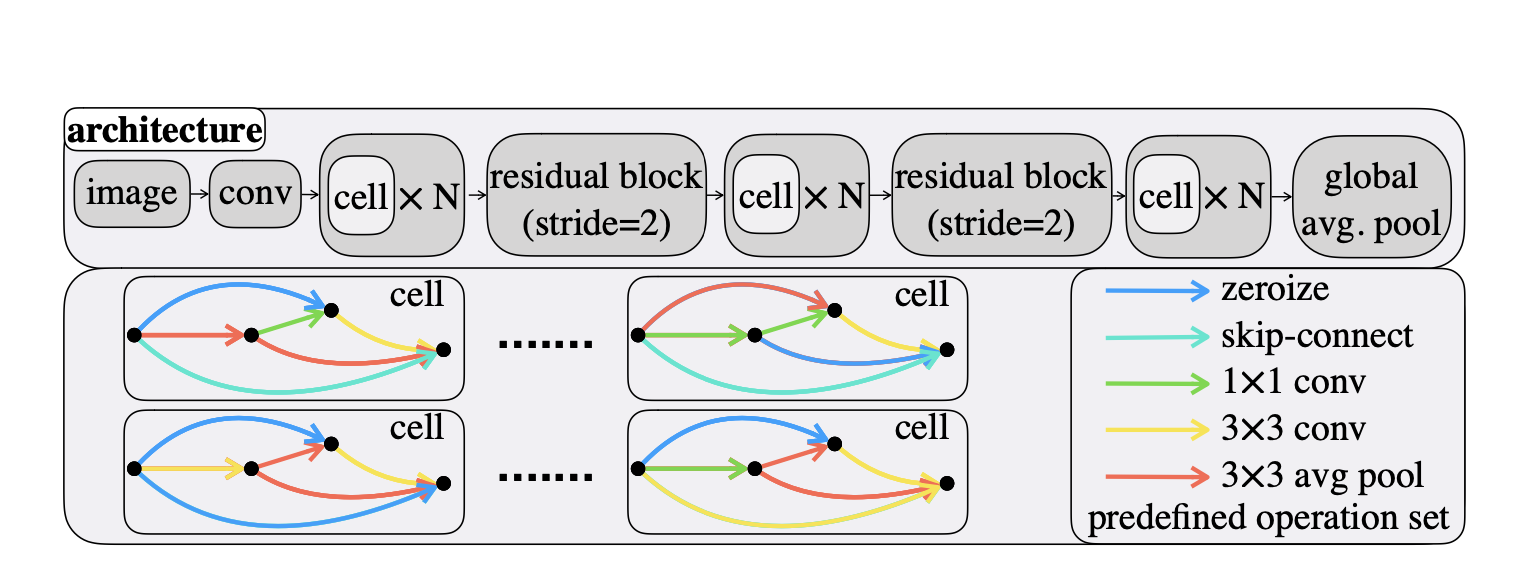
\includegraphics[scale=0.45]{figs/nas_bench_201.png}
		\refstepcounter{figure}
   		\addcontentsline{lof}{figure}{Figure~\thefigure: Illustration of the overall network architecture structure in NAS-Bench-201}
		\label{fig: nasbench201}
			\parbox{\linewidth}{
	 		\vspace{0.5em}
 	 		{\small \textit{Figure \ref{fig: nasbench201}:} Illustration of the skeleton (top) and the design of individual cells (bottom) of architectures in NAS-Bench-201 \cite{dong2020nasbench201}.
 	 		}
 		}
		\end{figure}

\vspace{0.5em}

Architectures in the search space are evaluated on three datasets that are widely used for image classification tasks: CIFAR-10, CIFAR-100 \cite{krizhevsky2009learning} and ImageNet-16-120 \cite{chrabaszcz2017downsampled}. Each dataset is split into the training, validation, and test sets and NAS-Bench-201 provides the training, validation, and test losses as well as accuracies for all architectures in the search space. We give a brief introduction to these datasets:

\begin{description}[leftmargin=0cm, listparindent=\parindent]
 	\item[CIFAR10]:	The dataset consists of 60K $32\times32$ color images in 10 classes. In NAS-Bench-201, 25K images with 10 classes are assigned into the training and the validation sets, respectively. The test set contains 10K images, with 1K images per class.
 	\item[CIFAR100]: This dataset has the same images as CIFAR-10 but in 100 classes. The training set has 50K images, and each of the validation and the test sets has 5K images.
 	\item[ImageNet-16-120]: This dataset contains 151.7K training images, 3K validation images, and 3K test images with 120 classes. Each image has 16$\times$16 pixels.
\end{description} 


NAS-Bench-201 has contributed to the \gls{nas} community in several aspects. First, it offers the assess to precomputed performance metrics for all architectures, allowing subsequent research to focus on the core search algorithm. With a unified dataset splitting strategy, it also enables consistent comparisons across different \gls{nas} algorithms. Additionally, NAS-Bench-201 serves as a foundation for extending benchmark datasets. For example, \cite{jung2023neural} introduces a dataset for benchmarking the robustness of neural networks.

In this work, we leverage the API offered by NAS-Bench-201 and directly query the performance metrics of the pre-trained architectures. In addition, NAS-Bench-201 also provides several analytical metrics, e.g., model ranking and accuracy correlations across the three datasets, which further guides our post-hoc analysis of the observed results.
